\section{Motivation}
\label{sec:motivation}

%Networking hardware is steadily getting faster. Today, NICs can transmit
%packets at a rate of 200~Gbps with latencies as low as
%600~ns~\cite{cx6-2018}. Similarly, DRAM capacities have been steadily
%increasing, with todays servers packing as much as 1~TB. Research
%leveraging these two trends has produced extremely fast and responsive
%storage systems. Using custom networking software (kernel-bypass) and
%by reliably storing all data in DRAM, these systems provide access
%latencies of a few microseconds while serving millions of operations per
%second.

%\subsection{Why Push Compute To Storage?}

%Trends in RAM density and network bandwidth and latency have led to a
%    wealth of research in extremely high-throughput and low-latency storage
%    systems.
Splinter's key motivation is the desire to support complex 
    data models and operations over large structures in a fast kernel-bypass
    stores.
Existing in-memory stores trade data model for performance by
  providing a simple key-value interface that only supports \texttt{get} and
  \texttt{put}.
Many real applications organize their data as trees, graphs, matrices, or vectors.
Performing operations like aggregation or tree traversal with a
  key-value interface often requires multiple \texttt{get}s.
Applications are usually \textsl{disaggregated} into a storage and
  compute tier, so these extra \texttt{get}s move data over the network
  and induce stalls for each request.

% Tree traversal.
\begin{figure}[t]
\centering
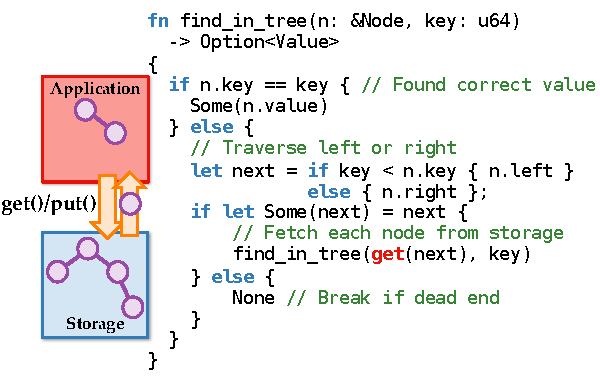
\includegraphics[width=1.0\columnwidth]{figures/sandstorm-tree-traversal.pdf}
\caption{Tree traversal using \texttt{get()} operations over a key-value
	store. Each step requires a lookup at the
	storage layer, which is latency-bound and expensive for deep traversals.
  If multitenant stores could be safely extended this function could avoid
  remote access stalls and request processing costs.}
\label{fig:kv-tree-traversal}
\end{figure}


Figure~\ref{fig:kv-tree-traversal} illustrates this problem with a
storage client that traverses data logically organized as a tree.
The client must first issue
a \texttt{get} to retrieve the tree's root node.
Next, it must perform a comparison and move down the tree by
issuing another \texttt{get}. It must repeat this
for every step of the traversal. Each \texttt{get} incurs a
round trip that fetches a single node from storage; since
the control flow is dependent on the data fetched, the client can only issue
one request at a time. The
number of round trips needed is proportional to the tree's depth, and a
significant portion of the tree gets moved over the network. Even with
modern low-latency networking, latency still dominates the client's performance:
network transmission and processing takes tens of
microseconds while the actual comparisons take less than a
microsecond~\cite{ramcloud}.

One solution is to customize the storage tier of each application to
support specialized data types. However, to improve efficiency and
utilization, storage tiers are usually deployed as multi-tenant
services~\cite{bigtable-2008,dynamo}, so they cannot be
customized for every possible data structure.
SQL could be used at the storage tier, but SQL is known to be a poor fit for data
types like graphs and matrices, does not support abstract data types,
and is too expensive at microsecond timescales. Instead,
Splinter takes a different approach;
it allows applications to push small pieces of native compute (extensions)
to stores at runtime. These extensions can
implement richer data types and operators, avoiding extra round trips
and reducing data movement.

\subsection{The Need for Lightweight Isolation}
Multi-tenancy at the storage layer makes running extensions challenging;
    a tenant cannot be allowed to access memory it does not own, starve
    others for resources, or crash the system.
The major challenge is that, at microsecond timescales, context switches and
    data copying across isolation boundaries significantly hurt performance.

% Table of context switch times (pre and post KPTI).
\begin{table}[t]
\centering
\begin{tabular}[]{l c c}
\toprule
\textbf{Xeon Architecture} & \multicolumn{2}{c}{\textbf{Context switch delay (\us)}} \\
\cline{2-3}
             & \textbf{Pre KPTI} & \textbf{KPTI} \\
\midrule
D-1548, Broadwell       & 1.60            & 2.40 \\
E5 2450, Sandy bridge   & 1.50            & 2.48 \\
Gold 6142, Skylake      & 1.40            & 2.16 \\
\bottomrule
\end{tabular}
\caption{Context switch overhead for different Intel Xeon
	architectures as measured on CloudLab. Each number represents
	the median of a million samples. Based on these measurements, we
	chose 2.16~\us and 1.40~\us for the context switch overhead with
	and without KPTI in our simulations.}
\label{table:context_switch}
\end{table}

To quantify the overhead of hardware isolation, we simulated an
  8-core multi-tenant store that isolates extensions using
  processes while varying the numbers of tenants making requests to it.
Simulated requests consume 1.5~\us of compute at the store; this
  is based on our benchmarks of simple unisolated operations on Splinter
  (\S\ref{sec:isolation-overhead}); our numbers are similar to those reported
  by others' kernel-bypass stores~\cite{ramcloud}.
Different context switch costs are simulated to show the
  overheads of hardware-based isolation of tenant code.
The simulation only accounts for context switch costs;
copying data across hardware isolation boundaries has also been shown to have
  significant performance costs~\cite{netbricks-2016}.
Nearly all extensions will access data, which will force data copying
  when using hardware isolation and hurt throughput further.
Based on measurements we made on different processor microarchitectures
  (Table~\ref{table:context_switch}), we simulate
  1.40~\us of overhead for a basic context switch and 2.16~\us for a
  KPTI~\cite{kpti-2018} protected kernel (which mitigates attacks
  that can leak the contents of protected memory~\cite{meltdown-2018}).
The request pattern is uniform;
all tenants make the same number of requests. The results are similar
  with skew.
The simulator is also optimistic; whenever a request is made and an idle core
  is available at the store that last processed a request from the same tenant,
  the isolation cost is assumed to be zero.

% Simulator graph (throughput vs number of tenants).
\begin{figure}[t]
\centering
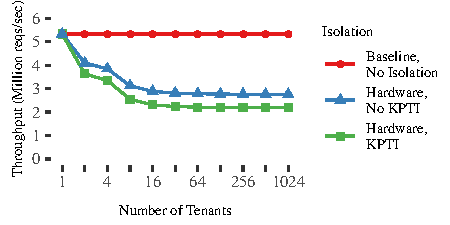
\includegraphics[width=1.0\columnwidth]{graphs/simulator.pdf}
\caption{Simulated throughput versus the number of tenants. With
	hardware isolation, even modestly increasing the number of
  tenants to 16 (just twice the number
	of cores) leads to a significant drop in throughput.
  ``No isolation'' represents an upper bound where isolation costs are zero.}
\label{fig:simulator}
\end{figure}


Figure~\ref{fig:simulator} presents simulated throughput at different
tenant densities. The baseline represents an upper bound where
extensions are run un-isolated at the storage system. The simulations
show that throughput with hardware isolation (irrespective of KPTI) is
significantly lower than the baseline. Even at just 16 tenants, context
switch costs alone cut server throughput by a factor of 1.8.
% Data for this statement: 8 cores
% 1500 ns processing time per req +
% 0 context switch overhead = 5.3e6
% 1400 context switch overhead = 2.97e6
% 2160 context switch overhead = 2.39e6

Overall, for these types of fast stores, hardware isolation limits performance
  and tenant density.
The challenges that we face in Splinter, and our design goals, stem from
    the need to (nearly)
  eliminate trust boundary crossing costs, to keep data movement across trust
  boundaries low, and to perform efficient fine-grained task scheduling.

